\section{Filter in der Bildverarbeitung \dcfirstauthorshort} \label{sec:filter}

Das Ziel in der Bildverarbeitung ist meist die Extraktion von Informationen bzw. die Erkennung von Objekten. In unserem Fall gilt es hauptsächlich herauszufinden, an welcher Stelle sich Linien im Bild befinden, die zur Fahrspur gehören. Hierbei kann das Graustufenbild als Matrix verstanden werden, deren Einträge die Helligkeit der einzelnen Pixel darstellen. 

Um bestimmte Eigenschaften zu ändern oder Informationen in einem Bild hervorzuheben, werden mathematische Operationen auf die Pixelmatrix angewendet. Diese Verfahren, deren Ergebnisse wieder ein Bild sind, teilen sich in Punktoperationen, Nachbarschaftsoperationen und globale Operationen auf \autocite[S.~111]{jaehneDigitaleBildverarbeitungMit2005}. Da Punktoperationen für jedes Pixel den Farb- oder Helligkeitswert neu berechnen, verwendet man sie typischerweise zur Korrektur von Kontrast, Helligkeit oder Farbraum. 

Objekte, wie zum Beispiel eine Straßenmarkierung, zeichnen sich meist dadurch aus, dass sich Pixel in Merkmalen von ihren Nachbarpixeln unterscheiden. Bei den Nachbarschaftsoperationen berechnen sich die Werte der Pixel des neuen Bildes aus den Bildpunkten einer kleinen Umgebung um die Punkte. Weil durch eine Nutzung des Nachbarschaftsoperators das Bild verändert wird und Informationen generell verloren gehen, spricht man auch von einem \emph{Filter}. 

Das von uns verwendete und sehr verbreitete Faltungsfilter verrechnet zur Ergebnisbildung die Helligkeitswerte über einen Filterkern miteinander. Der Filterkern ist hierbei eine quadratische, symmetrische Matrix, die mit der Pixelmatrix des Bildes gefaltet wird. Die Faltung zweier Funktionen beschreibt den durch eine andere Funktion gewichteten Mittelwert einer Funktion. Unter dem Faltungsprodukt \( \mathrm{f_1}(\gls{lat:time}) \ast \mathrm{f_2}(\gls{lat:time}) \) zweier Originalfunktionen \(\mathrm{f_1}(\gls{lat:time}) \) und \(\mathrm{f_2}(\gls{lat:time}) \) versteht man allgemein das Integral \autocite[S.~584]{papulaMathematikFuerIngenieure2012}

% allgemeine Faltungsformel
\begin{equation}
\mathrm{f_1}(\gls{lat:time}) \ast \mathrm{f_2}(\gls{lat:time}) = \int \limits_{-\infty}^{+\infty} \mathrm{f_1}(\scl{\tau}) \cdot \mathrm{f_2}(\gls{lat:time}-\scl{\tau})d\scl{\tau}
\end{equation}

 Die Bildmatrix und der Filterkern sind jedoch diskrete Funktionen. Deswegen wird das Integral zu einer Summe. Seien \(\mtx{M}^{\ast}\) das gefilterte, \mtx{M} das originale Bild, \mtx{F} der Filterkern, \scl{k} und \scl{l} dessen Matrixdimensionen und (\scl{o_x},\scl{o_y}) der Mittelpunkt des Filterkerns, dann ergibt sich folgende Berechnungsformel für die diskrete Faltung \autocite{cabfdbFaltungsmatrixWikipedia2010}:

% Formel diskrete Faltung:
\begin{equation}
\mtx{M}^{\ast}(\gls{x},\gls{y}) = \sum_{\scl{i}=1}^{\scl{k}} \sum_{\scl{j}=1}^{\scl{l}} \mtx{M}(\gls{x}-\scl{i}+\scl{o_x}, \gls{y}-\scl{j}+\scl{o_y}) \cdot \mtx{F}(\scl{i},\scl{j})
\end{equation}

Ein Faltungsfilter berechnet also den Wert des neuen Pixels aus dem gewichteten Mittelwert der umliegenden Pixel innerhalb des Filterkerns. Je nachdem, nach welcher Funktion gewichtet wird, ergibt sich der Name des Filters und was er in dem Bild verändert. 
%In dieser Arbeit wurden das Gauß-Filter zum Glätten und das Laplace-Filter zur Kanten- und letztlich Liniendetektion genutzt.

Um Rechenzeit mit einem zweidimensionalen Filter einzusparen, existiert die Möglichkeit, ihn so in zwei eindimensionale Operatoren zu zerlegen, dass deren Matrixmultiplikation wieder den ursprünglichen 2D-Filter ergibt (\ref{eq:grundlagen_filter_separierbarkeit}, aus \autocite[S.~123]{jaehneDigitaleBildverarbeitungMit2005}). 

\begin{equation}
\begin{pmatrix}
1 & 4 	& 6		& 4 	& 1 	\\
4 & 16 	& 24	& 16 	& 4 	\\
6 & 24	& 36	& 24	& 6    	\\
4 & 16 	& 24	& 16	& 4		\\
1 & 4	& 6		& 4		& 1		\\	
\end{pmatrix}
=
\begin{pmatrix}
1 & 4 	& 6		& 4 	& 1 	\\
\end{pmatrix}
\cdot
\begin{pmatrix}
1 \\
4 \\
6 \\
4 \\
1 \\	
\end{pmatrix}
\label{eq:grundlagen_filter_separierbarkeit}
\end{equation}

Wenn dies möglich ist, nennt man das Filter \emph{separierbar}. Die Anwendung des zweiten Operators auf das Zwischenergebnis des ersten auf das Bild hat das gleiche Ergebnis zur Folge, führt jedoch zu einem geringeren Rechenaufwand.

\subsection{Gauß-Filter}

Der Filterkern des Gauß-Filters stellt sich aus der Dichtefunktion \( \mathrm{h} \) der Normalverteilung auf (\glqq Gaußsche Glockenkurve\grqq, \autocite[S.~371]{papulaMathematikFuerIngenieure2016}).

% Formel für Dichtefunktion h
\begin{equation}
\mathrm{h}(\gls{x}) = \frac{1}{\gls{gre:standartabweichung} \sqrt{2 \gls{gre:pi}}} \cdot \gls{lat:eulnum}^{-\frac{{\gls{x}}^2}{2{\gls{gre:standartabweichung}}^2}}
%\label{eq:gaussfkt}
\end{equation}

Dieses Filter ist ein Tiefpassfilter und wird zur Glättung und zum Weichzeichnen verwendet. Hierbei wird angenommen, dass das Bildrauschen normalverteilt ist. Jenes kann mit diesem Filter vermindert werden. Die zu diskretisierende Filterfunktion \( \mathrm{h}_2 \) in zwei Dimensionen ergibt sich, wenn man die Dichtefunktionen beider Richtungen \gls{x} und \gls{y} miteinander multipliziert.

% Formel für Gauß-Funktion (Impulsantwort bei zwei Dimensionen)
\begin{equation}
\mathrm{h}_2(\gls{x},\gls{y}) = \mathrm{h}(\gls{x}) \cdot \mathrm{h}(\gls{y}) = \frac{1}{2 {\gls{gre:pi} \gls{gre:standartabweichung}}^2} \cdot \gls{lat:eulnum}^{-\frac{{\gls{x}}^2+{\gls{y}}^2}{2{\gls{gre:standartabweichung}}^2}}
%\label{eq:gaussfkt}
\end{equation}

Mit dem Zusammenspiel von der Filterkerngröße und der Standartabweichung \gls{gre:standartabweichung} lässt sich einstellen, wie stark das Bild verwischt. Je größer der Kern und \gls{gre:standartabweichung} sind, desto verschwommener ist das Resultat. In Abbildung~\ref{fig:grundlagen_gaussfilter} ist beispielhaft ein \( 15\times15\) - Filterkern mit \( \gls{gre:standartabweichung} = 3\) dargestellt.

\begin{figure}[H] % [htb]
  \centering
  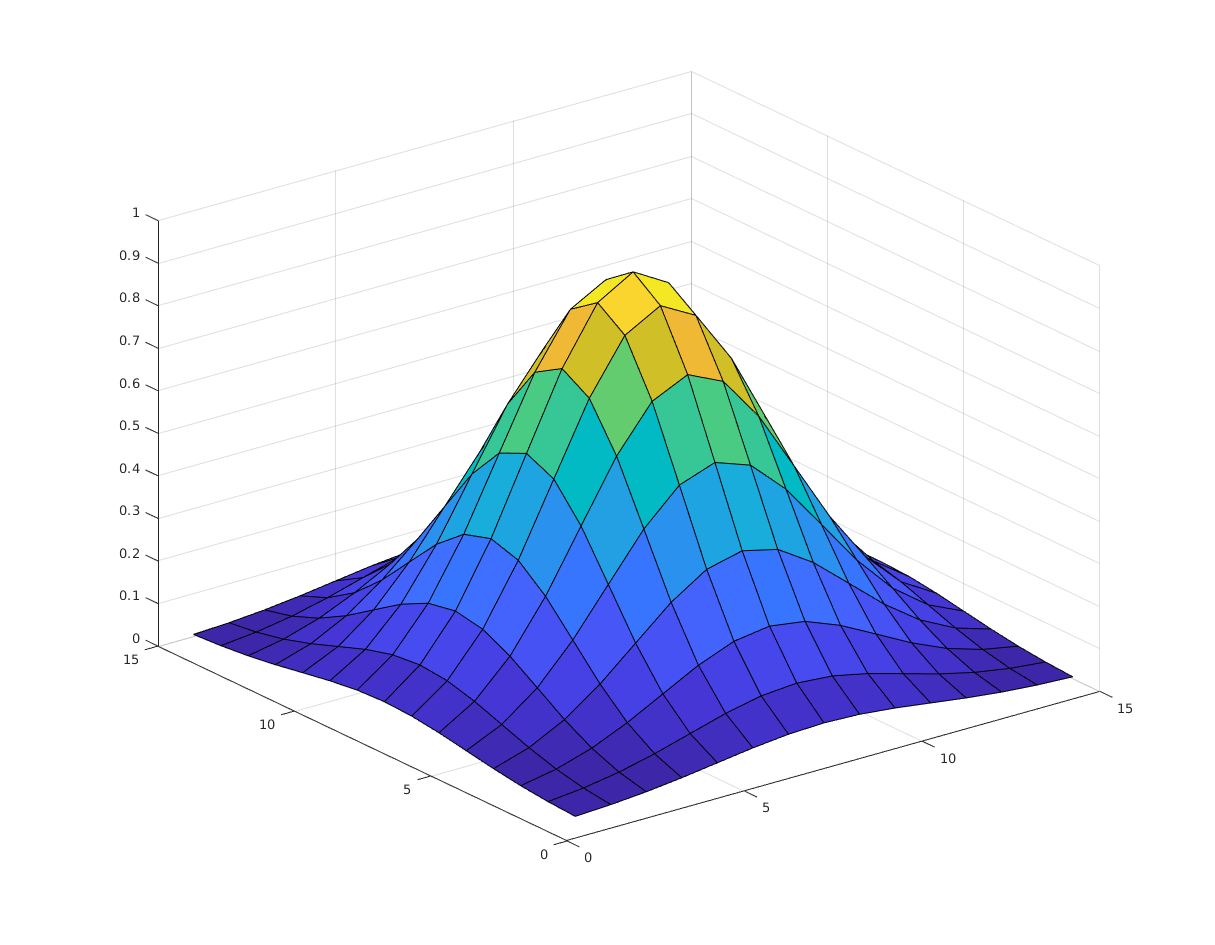
\includegraphics[width=0.9\textwidth]{grundlagen_gaussfilter.png}
  \caption{3D-Plot der Matrix eines \( 15\times15\) - Gauß-Filters}
  \label{fig:grundlagen_gaussfilter}
\end{figure}  

\subsection{Laplace-Filter} \label{ssec:laplaceFilter}
% welcher starke Veränderungen in den Helligkeitsunterschieden zu benachbarten Pixeln hervorhebt.
%In der zweiten Ableitung sind Kanten die Nulldurchgänge 

Möchte man in einem Bild Kanten detektieren, basiert die Lösung des Problems meist auf Ableitungen verschiedenen Grades \autocite[S.~360ff]{jaehneDigitaleBildverarbeitungMit2005}. (In der ersten Ableitung sind Kanten z.B. die Extremstellen.) Ein Filter zur Kantendetektion sollte Diskontinuitäten in den Grauwerten hervorheben und konstante Grauwerte unterdrücken. Der Laplace-Filter, bzw. diskrete Laplace-Operator, nutzt dafür die Summe der partiellen zweiten Ableitungen in alle Richtungen. \autocite[S.~90]{papulaMathematikFuerIngenieure2016}

% Formel für den Laplace-Operator
\begin{equation}
\Delta \mathrm{f} = \frac{\partial^2 \mathrm{f}}{\partial {\gls{x}}^2} + \frac{\partial^2 \mathrm{f}}{\partial {\gls{y}}^2}
\end{equation}

% Die gesuchten Kanten sind dann die Nulldurchgänge in der zweiten Ableitung, vor und nach denen es unmittelbar Signalspitzen gibt, die höher als das Rauschen sind. 
Die Nulldurchgänge, vor und nach denen es unmittelbar Signalspitzen gibt, sind dann die gesuchten Kanten. Ein großer Nachteil dieser Filtermethode ist das relativ stark verrauschte Ergebnisbild.

Eine spezielle Form eines diskreten Laplace-Filters ist der \gls{acr:log}, welcher in dieser Arbeit zur Liniendetektion genutzt wurde. Der in Abbildung~\ref{fig:grundlagen_logfilter} beispielhaft dargestellte Filterkern wird durch die Anwendung des Laplace-Operators auf eine Gaußfunktion erstellt. Dieses Filter bewirkt neben der Kantendetektion eine gaußsche Glättung und mindert so das störende Rauschen.

\begin{figure}[H] % [htb]
  \centering
  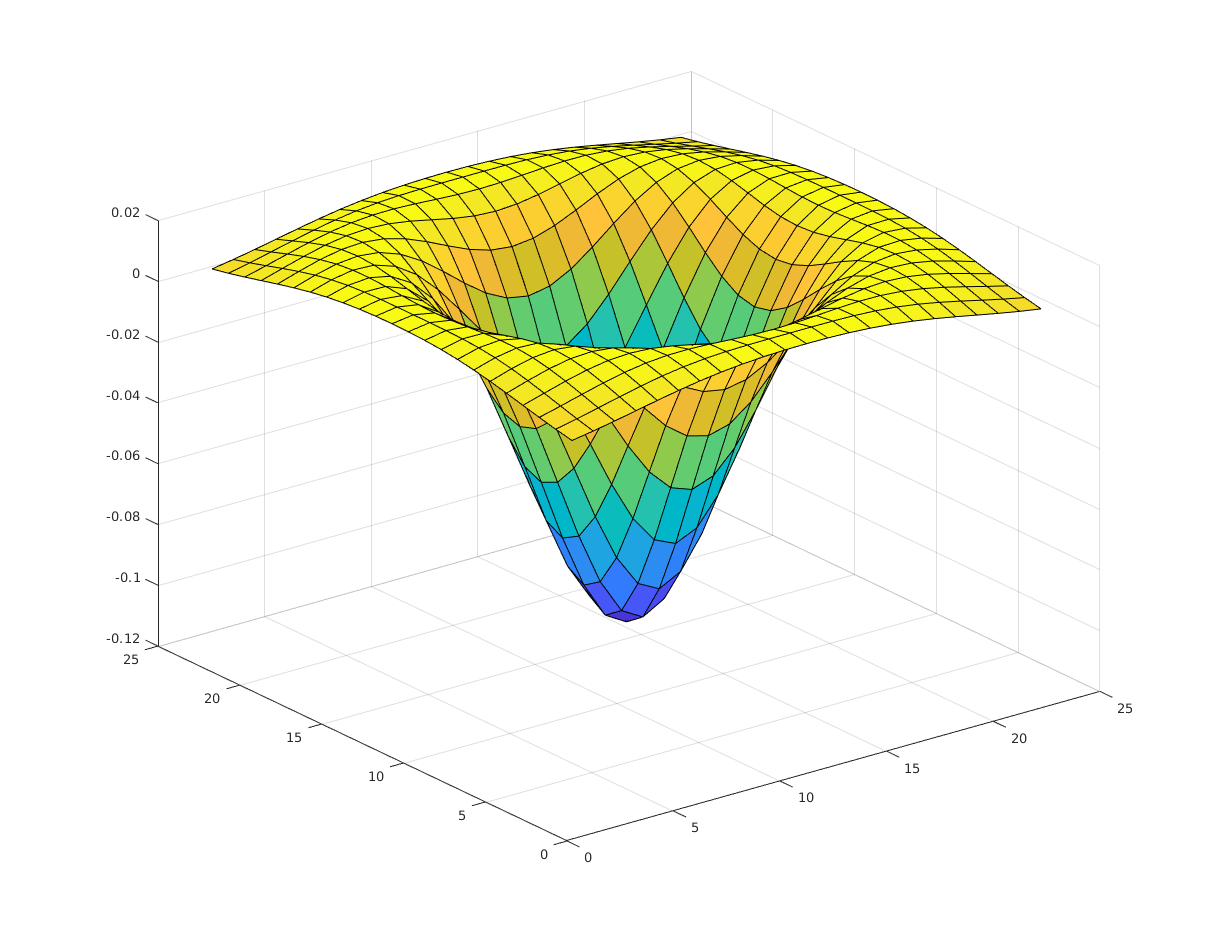
\includegraphics[width=0.9\textwidth]{grundlagen_logfilter.png}
  \caption{3D-Plot der Matrix eines \( 23\times23\) - \gls{acr:log}-Filters}
  \label{fig:grundlagen_logfilter}
\end{figure}  

